\documentclass[border=14pt]{standalone}
\usepackage[T1]{fontenc}
\usepackage[default]{sourcesanspro}
\usepackage{tikz}
\usetikzlibrary{arrows.meta}

% Blank coordinate system for Exercise 1
%   x-axis: Stunden Schlaf (0..10)
%   y-axis: Prüfungsnote   (0..6)
%   Scale: x=0.8cm per unit, y=0.8cm per unit

\begin{document}
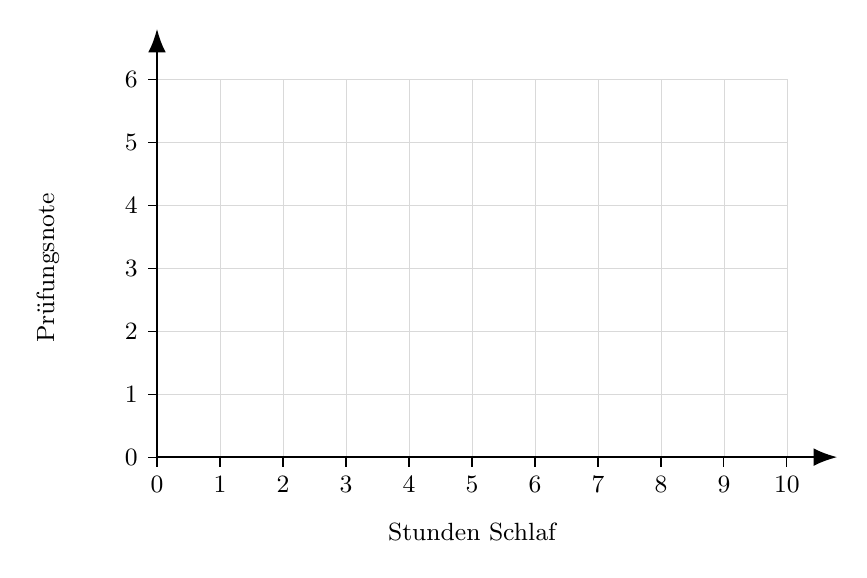
\begin{tikzpicture}[x=0.8cm, y=0.8cm]

  % --- Grid ---
  \draw[step=1, gray!30, very thin] (0,0) grid (10,6);

  % --- Axes ---
  \draw[thick,-{Latex[length=3mm]}] (0,0) -- (10.8,0);
  \draw[thick,-{Latex[length=3mm]}] (0,0) -- (0,6.8);

  % --- X ticks ---
  \foreach \x in {0,...,10} {
    \draw (\x, 0) -- (\x, -0.15) node[below, font=\small] {\x};
  }
  \node[font=\small, anchor=north] at (5, -0.9) {Stunden Schlaf};

  % --- Y ticks ---
  \foreach \y in {0,...,6} {
    \draw (0, \y) -- (-0.15, \y) node[left, font=\small] {\y};
  }
  \node[font=\small, rotate=90, anchor=south] at (-1.4, 3) {Prüfungsnote};

\end{tikzpicture}
\end{document}
